\section{Risk Heatmap}

\begin{exhibitbox}[Exhibit 35: Probability-impact heatmap]
\centering
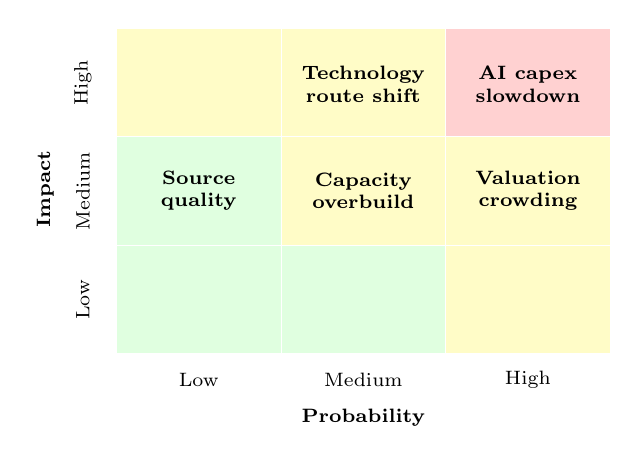
\begin{tikzpicture}[scale=0.95]
\foreach \x/\xlabel in {0/Low,1/Medium,2/High} {
  \node[font=\scriptsize] at (\x*2.2+1.1,-0.35) {\xlabel};
}
\foreach \y/\ylabel in {0/Low,1/Medium,2/High} {
  \node[font=\scriptsize, rotate=90] at (-0.45,\y*1.45+0.72) {\ylabel};
}
\node[font=\scriptsize\bfseries] at (3.3,-0.85) {Probability};
\node[font=\scriptsize\bfseries, rotate=90] at (-0.95,2.2) {Impact};
\foreach \x in {0,1,2} {
  \foreach \y in {0,1,2} {
    \pgfmathtruncatemacro{\score}{\x+\y}
    \ifnum\score<2 \def\fillc{green!12}\else\ifnum\score<4 \def\fillc{yellow!22}\else\def\fillc{red!18}\fi\fi
    \draw[fill=\fillc, draw=white] (\x*2.2,\y*1.45) rectangle ++(2.2,1.45);
  }
}
\node[align=center, font=\scriptsize\bfseries, text width=2cm] at (5.5,3.6) {AI capex\\slowdown};
\node[align=center, font=\scriptsize\bfseries, text width=2cm] at (5.5,2.18) {Valuation\\crowding};
\node[align=center, font=\scriptsize\bfseries, text width=2cm] at (3.3,3.6) {Technology\\route shift};
\node[align=center, font=\scriptsize\bfseries, text width=2cm] at (3.3,2.18) {Capacity\\overbuild};
\node[align=center, font=\scriptsize\bfseries, text width=2cm] at (1.1,2.18) {Source\\quality};
\end{tikzpicture}
\sourcenote{\texttt{risk\_framework.md}}
\end{exhibitbox}

\section{Risk Trigger Matrix}

\begin{exhibitbox}[Exhibit 36: What would make us change the view]
\footnotesize
\begin{tabularx}{\textwidth}{L{2.4cm}X X X}
\toprule
\textbf{Risk} & \textbf{Why it matters} & \textbf{Observable trigger} & \textbf{Action} \\
\midrule
AI资本开支放缓 & 多数多头逻辑依赖云厂商CAPEX、NVIDIA升级和ASIC服务器扩张。 & CSP下修CAPEX、AI服务器订单延期、PCB在手订单走弱。 & 高弹性PCB从核心/进攻降为观察。 \\
技术路线迁移 & CoWoP、玻璃基板、光互联、铜缆、mSAP会重新分配价值池。 & 新平台减少板级价值或材料规格变化。 & 重新拆分PCB/载板/封装/光互联价值量。 \\
产能过剩 & 高CAPEX若遇需求放缓，将带来价格竞争。 & 利用率下降、交期缩短、价格松动但CAPEX继续上升。 & 下调情景倍数，要求订单验证。 \\
估值拥挤 & 若干标的已反映强兑现预期。 & 股价上涨快于盈利预测上修，PE超过增长支撑。 & 触发器跟踪，避免无条件乐观。 \\
\bottomrule
\end{tabularx}
\end{exhibitbox}

\section{Monitoring Checklist}

\begin{dashboardbox}[Monitoring dashboard]
\small
\begin{tabularx}{\textwidth}{L{3cm}X L{3cm}}
\toprule
\textbf{Monitor} & \textbf{Signal} & \textbf{Frequency} \\
\midrule
AI平台节奏 & Rubin/Rubin Ultra、ASIC服务器、交换机和光模块放量时间表。 & Monthly / event-driven \\
订单与CAPEX & PCB龙头在手订单、利用率、扩产计划、设备订单。 & Quarterly \\
材料价格 & M8/M9 CCL价格、交期、客户认证和原材料成本。 & Monthly \\
财务兑现 & 收入增速、毛利率、费用率、经营现金流和折旧压力。 & Quarterly \\
技术替代 & 玻璃基板、光互联、铜缆和新背板架构是否改变PCB价值池。 & Event-driven \\
\bottomrule
\end{tabularx}
\end{dashboardbox}

\section{Invalidation Conditions}

\begin{riskbox}[Invalidation conditions / 失效条件]
若出现以下任一情况，本报告的核心跟踪框架需要下修或重做：
\begin{itemize}
  \item AI服务器、ASIC或高速交换机资本开支连续两个季度低于预期，同时核心公司订单/产能利用率转弱。
  \item M8/M9等高端CCL涨价和交期紧张逆转，且材料厂毛利率无法维持。
  \item 核心标的在收入高增的同时经营现金流、毛利率或在手订单显著背离，说明需求兑现质量不足。
  \item 玻璃基板、CPO或其它互联架构实质性转移PCB/CCL价值池，导致本报告的价值链映射失效。
  \item 官方披露或可信原始报告否定当前平台链代理关系或关键技术路线。
\end{itemize}
\end{riskbox}
